\documentclass[
  shownotes,
  xcolor={svgnames},
  hyperref={colorlinks,citecolor=DarkBlue,linkcolor=DarkRed,urlcolor=DarkBlue}
  , aspectratio=169]{beamer}
\usepackage{animate}
\usepackage{amsmath}
\usepackage{amsfonts}
\usepackage{amssymb}
\usepackage{pifont}
\usepackage{mathpazo}
%\usepackage{xcolor}
\usepackage{multimedia}
\usepackage{fancybox}
\usepackage[para]{threeparttable}
\usepackage{multirow}
\setcounter{MaxMatrixCols}{30}
\usepackage{subcaption}
\usepackage{graphicx}
\usepackage{lscape}
\usepackage[compatibility=false,font=small]{caption}
\usepackage{booktabs}
\usepackage{ragged2e}
\usepackage{chronosys}
\usepackage{appendixnumberbeamer}
\usepackage{animate}
\setbeamertemplate{caption}[numbered]
\usepackage{color}
%\usepackage{times}
\usepackage{tikz}
\usepackage{comment} %to comment
%% BibTeX settings
\usepackage{natbib}
\bibliographystyle{apalike}
\bibpunct{(}{)}{,}{a}{,}{,}
\setbeamertemplate{bibliography item}{[\theenumiv]}

% Defines columns for bespoke tables
\usepackage{array}
\newcolumntype{L}[1]{>{\raggedright\let\newline\\\arraybackslash\hspace{0pt}}m{#1}}
\newcolumntype{C}[1]{>{\centering\let\newline\\\arraybackslash\hspace{0pt}}m{#1}}
\newcolumntype{R}[1]{>{\raggedleft\let\newline\\\arraybackslash\hspace{0pt}}m{#1}}


\usepackage{xfrac}


\usepackage{multicol}
\setlength{\columnsep}{0.5cm}

% Theme and colors
\usetheme{Boadilla}

% I use steel blue and a custom color palette. This defines it.
\definecolor{andesred}{HTML}{af2433}

% Other options
\providecommand{\U}[1]{\protect\rule{.1in}{.1in}}
\usefonttheme{serif}
\setbeamertemplate{itemize items}[default]
\setbeamertemplate{enumerate items}[square]
\setbeamertemplate{section in toc}[circle]

\makeatletter

\definecolor{mybackground}{HTML}{82CAFA}
\definecolor{myforeground}{HTML}{0000A0}

\setbeamercolor{normal text}{fg=black,bg=white}
\setbeamercolor{alerted text}{fg=red}
\setbeamercolor{example text}{fg=black}

\setbeamercolor{background canvas}{fg=myforeground, bg=white}
\setbeamercolor{background}{fg=myforeground, bg=mybackground}

\setbeamercolor{palette primary}{fg=black, bg=gray!30!white}
\setbeamercolor{palette secondary}{fg=black, bg=gray!20!white}
\setbeamercolor{palette tertiary}{fg=white, bg=andesred}

\setbeamercolor{frametitle}{fg=andesred}
\setbeamercolor{title}{fg=andesred}
\setbeamercolor{block title}{fg=andesred}
\setbeamercolor{itemize item}{fg=andesred}
\setbeamercolor{itemize subitem}{fg=andesred}
\setbeamercolor{itemize subsubitem}{fg=andesred}
\setbeamercolor{enumerate item}{fg=andesred}
\setbeamercolor{item projected}{bg=gray!30!white,fg=andesred}
\setbeamercolor{enumerate subitem}{fg=andesred}
\setbeamercolor{section number projected}{bg=gray!30!white,fg=andesred}
\setbeamercolor{section in toc}{fg=andesred}
\setbeamercolor{caption name}{fg=andesred}
\setbeamercolor{button}{bg=gray!30!white,fg=andesred}


\usepackage{fancyvrb}
\newcommand{\VerbBar}{|}
\newcommand{\VERB}{\Verb[commandchars=\\\{\}]}
\DefineVerbatimEnvironment{Highlighting}{Verbatim}{commandchars=\\\{\}}
% Add ',fontsize=\small' for more characters per line
\usepackage{framed}
\definecolor{shadecolor}{RGB}{248,248,248}
\newenvironment{Shaded}{\begin{snugshade}}{\end{snugshade}}
\newcommand{\AlertTok}[1]{\textcolor[rgb]{0.94,0.16,0.16}{#1}}
\newcommand{\AnnotationTok}[1]{\textcolor[rgb]{0.56,0.35,0.01}{\textbf{\textit{#1}}}}
\newcommand{\AttributeTok}[1]{\textcolor[rgb]{0.77,0.63,0.00}{#1}}
\newcommand{\BaseNTok}[1]{\textcolor[rgb]{0.00,0.00,0.81}{#1}}
\newcommand{\BuiltInTok}[1]{#1}
\newcommand{\CharTok}[1]{\textcolor[rgb]{0.31,0.60,0.02}{#1}}
\newcommand{\CommentTok}[1]{\textcolor[rgb]{0.56,0.35,0.01}{\textit{#1}}}
\newcommand{\CommentVarTok}[1]{\textcolor[rgb]{0.56,0.35,0.01}{\textbf{\textit{#1}}}}
\newcommand{\ConstantTok}[1]{\textcolor[rgb]{0.00,0.00,0.00}{#1}}
\newcommand{\ControlFlowTok}[1]{\textcolor[rgb]{0.13,0.29,0.53}{\textbf{#1}}}
\newcommand{\DataTypeTok}[1]{\textcolor[rgb]{0.13,0.29,0.53}{#1}}
\newcommand{\DecValTok}[1]{\textcolor[rgb]{0.00,0.00,0.81}{#1}}
\newcommand{\DocumentationTok}[1]{\textcolor[rgb]{0.56,0.35,0.01}{\textbf{\textit{#1}}}}
\newcommand{\ErrorTok}[1]{\textcolor[rgb]{0.64,0.00,0.00}{\textbf{#1}}}
\newcommand{\ExtensionTok}[1]{#1}
\newcommand{\FloatTok}[1]{\textcolor[rgb]{0.00,0.00,0.81}{#1}}
\newcommand{\FunctionTok}[1]{\textcolor[rgb]{0.00,0.00,0.00}{#1}}
\newcommand{\ImportTok}[1]{#1}
\newcommand{\InformationTok}[1]{\textcolor[rgb]{0.56,0.35,0.01}{\textbf{\textit{#1}}}}
\newcommand{\KeywordTok}[1]{\textcolor[rgb]{0.13,0.29,0.53}{\textbf{#1}}}
\newcommand{\NormalTok}[1]{#1}
\newcommand{\OperatorTok}[1]{\textcolor[rgb]{0.81,0.36,0.00}{\textbf{#1}}}
\newcommand{\OtherTok}[1]{\textcolor[rgb]{0.56,0.35,0.01}{#1}}
\newcommand{\PreprocessorTok}[1]{\textcolor[rgb]{0.56,0.35,0.01}{\textit{#1}}}
\newcommand{\RegionMarkerTok}[1]{#1}
\newcommand{\SpecialCharTok}[1]{\textcolor[rgb]{0.00,0.00,0.00}{#1}}
\newcommand{\SpecialStringTok}[1]{\textcolor[rgb]{0.31,0.60,0.02}{#1}}
\newcommand{\StringTok}[1]{\textcolor[rgb]{0.31,0.60,0.02}{#1}}
\newcommand{\VariableTok}[1]{\textcolor[rgb]{0.00,0.00,0.00}{#1}}
\newcommand{\VerbatimStringTok}[1]{\textcolor[rgb]{0.31,0.60,0.02}{#1}}
\newcommand{\WarningTok}[1]{\textcolor[rgb]{0.56,0.35,0.01}{\textbf{\textit{#1}}}}
\usepackage{graphicx}
\makeatletter


% colors
\definecolor{airforceblue}{rgb}{0.36, 0.54, 0.66}
\newcommand{\theme}{\color{andesred}}
\newcommand{\bk}{\color{black}}
\newcommand{\rd}{\color{red}}
\newcommand{\fg}{\color{ForestGreen}}
\newcommand{\bl}{\color{blue}}
\newcommand{\gr}{\color{black!60}}
\newcommand{\sg}{\color{DarkSlateGray}}
\newcommand{\br}{\color{SaddleBrown}}
\newcommand{\nv}{\color{Navy}}


% common math markups
\newcommand{\bs}[1]{\boldsymbol{#1}}
\newcommand{\mc}[1]{\mathcal{#1}}
\newcommand{\mr}[1]{\mathrm{#1}}
\newcommand{\bm}[1]{\mathbf{#1}}
\newcommand{\ds}[1]{\mathds{#1}}
\newcommand{\indep}{\perp\!\!\!\perp}

% shorthand
\newcommand{\sk}{\vspace{.5cm}}
\newcommand{\R}[1]{{\tt \nv #1}}
\newcommand{\til}{{\footnotesize$\bs{\stackrel{\sim}{}}$}}
\DeclareSymbolFont{extraup}{U}{zavm}{m}{n}
\DeclareMathSymbol{\vardiamond}{\mathalpha}{extraup}{87}


\usepackage{tikz}
% Tikz settings optimized for causal graphs.
\usetikzlibrary{shapes,decorations,arrows,calc,arrows.meta,fit,positioning}
\tikzset{
    -Latex,auto,node distance =1 cm and 1 cm,semithick,
    state/.style ={ellipse, draw, minimum width = 0.7 cm},
    point/.style = {circle, draw, inner sep=0.04cm,fill,node contents={}},
    bidirected/.style={Latex-Latex,dashed},
    el/.style = {inner sep=2pt, align=left, sloped}
}


\makeatother






%%%%%%%%%%%%%%% BEGINS DOCUMENT %%%%%%%%%%%%%%%%%%

\begin{document}
 
\title[Lecture 27]{Lecture 27:   PCR and PLS}
\subtitle{Big Data and Machine Learning for Applied Economics \\ Econ 4676}
\date{\today}

\author[Sarmiento-Barbieri]{Ignacio Sarmiento-Barbieri}
\institute[Uniandes]{Universidad de los Andes}


\begin{frame}[noframenumbering]
\maketitle
\end{frame}

%%%%%%%%%%%%%%%%%%%%%%%%%%%%%%%%%%%




%----------------------------------------------------------------------% 

\begin{frame}
\frametitle{Agenda}

\tableofcontents

\end{frame}

%----------------------------------------------------------------------%
\section{Recap}
%----------------------------------------------------------------------%
\begin{frame}[fragile]
\frametitle{Recap: PCA serves as a dimentionality reduction technique }


\begin{itemize}

\item Eigenvalues and eigenvectors associated to the covariance matrix of the data $X_{n\times p}$, $V(X)=S_{p\times p}$
  
  \begin{align}
  \lambda_1 = \delta_1 S \delta'_1 
  \end{align}
\medskip
\item We get an ``index'' $f_s = \delta_s X$ : 'loadings' often suggest that a factor works as a 'index' of a group of variables.
\medskip
\item Important to scale the variables (sensible to units)
\medskip
\item Different criteria for choosing the number of PC

\begin{itemize}
  \item Visual examination of screeplot
  \item Kaiser criterion.
  \item Proportion of variance explained.
\end{itemize}
\end{itemize}

\end{frame}

%----------------------------------------------------------------------%
\begin{frame}[fragile]
\frametitle{Factor Interpretation: Example}


\begin{itemize}
\item {\bf Congress and \theme Roll Call Voting}
\bigskip
\begin{itemize}
  \item Votes in which names and positions are recorded are called `roll calls'.
  \medskip
  \item The site {\tt voteview.com} archives vote records and the R package { \tt pscl} has tools for this data.
  \medskip
  \item 445 members in the last US House  (the $111^{th}$)
  \medskip
  \item 1647 votes:  \theme nea = -1, \nv yea=+1, \gr missing = 0.
  \medskip
  \item This leads to a large matrix of observations that can probably be reduced to simple factors {\gr (party)}.
\end{itemize}
\end{itemize}





\end{frame}


%----------------------------------------------------------------------%
\begin{frame}[fragile]
\frametitle{Factor Interpretation}

\begin{itemize}

  \item Vote components in the $\bs{111^{th}}$ house
 
 \item Each PC is $f_s = \delta_s X$ 

  \begin{figure}[H] \centering
            \captionsetup{justification=centering}
              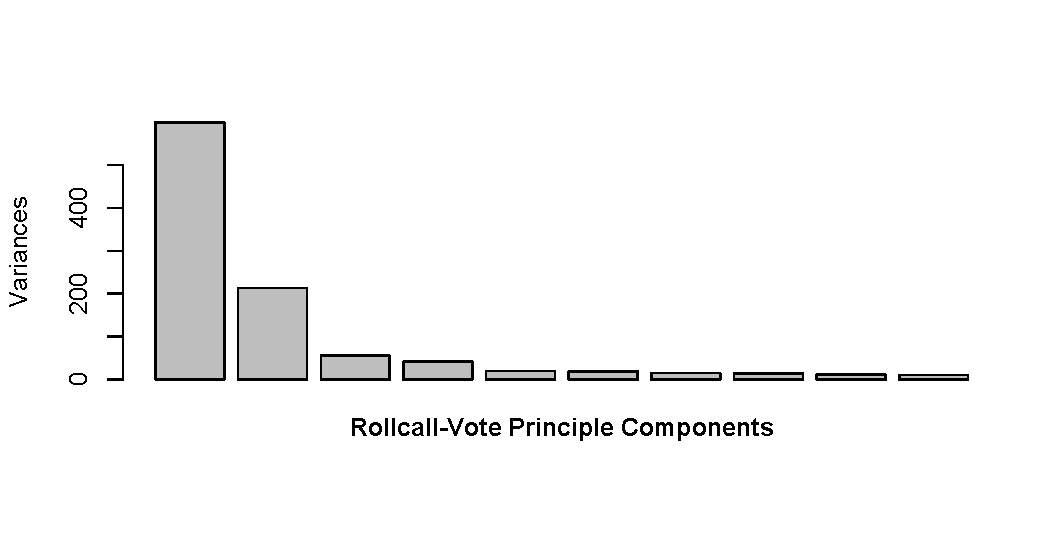
\includegraphics[scale=0.5]{../Lecture26/figures/VOTEscree}
              
 \end{figure}

\item Huge drop in variance from $1^{st}$ to $2^{nd}$ and  $2^{nd}$ to $3^{rd}$ PC.
\item Poli-Sci holds that PC1 is usually enough to explain congress. \\\sg 2nd component has been important twice: 1860's and 1960's.

\end{itemize}


\end{frame}

%----------------------------------------------------------------------%
\begin{frame}[fragile]
\frametitle{Factor Interpretation}

\begin{itemize}
\item Top two PC directions in the $\bs{111^{th}}$ house



  \begin{figure}[H] \centering
            \captionsetup{justification=centering}
              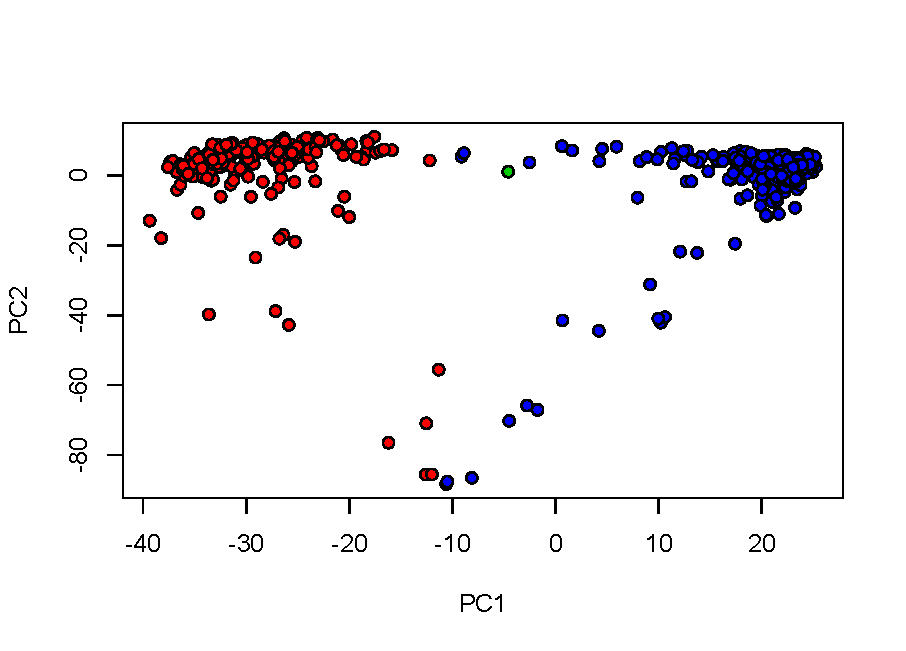
\includegraphics[scale=.5]{../Lecture26/figures/VOTEpc}
 \end{figure}




  \item Republicans in red and Democrats in blue: 
  \begin{itemize}
  \item Clear separation on the first principal component.
  \item The second component looks orthogonal to party.
  \end{itemize}
\end{itemize}


\end{frame}


%----------------------------------------------------------------------%
\begin{frame}[fragile]
\frametitle{Factor Interpretation}




{\scriptsize \nv

{\theme \tt \#\# Far right (very conservative) \vspace{-.25cm}}
\begin{verbatim}
> sort(votepc[,1])
     BROUN (R GA-10)       FLAKE (R AZ-6)   HENSARLIN (R TX-5) 
         -39.3739409          -38.2506713          -37.5870597 
\end{verbatim}

{\theme \tt \#\# Far left (very liberal) \vspace{-.25cm}}
\begin{verbatim}
> sort(votepc[,1], decreasing=TRUE)
    EDWARDS (D MD-4)   PRICE (D NC-4)    MATSUI (D CA-5)      
         25.2915083        25.1591151         25.1248117     
\end{verbatim}       
  

{\theme \tt \#\# social issues? immigration? no clear pattern\vspace{-.25cm}}
\begin{verbatim}
> sort(votepc[,2])
     SOLIS (D CA-32) GILLIBRAND (D NY-20)      PELOSI (D CA-8) 
        -88.31350926         -87.58871687         -86.53585568 
   STUTZMAN (R IN-3)       REED (R NY-29)      GRAVES (R GA-9) 
        -85.59217310         -85.53636319         -76.49658108 
\end{verbatim}
}

\begin{itemize}
  \item PC1 is easy to read, PC2 is ambiguous (is it even meaningful?)
\end{itemize}


\end{frame}
%----------------------------------------------------------------------%
\begin{frame}[fragile]
\frametitle{Factor Interpretation}

\begin{itemize}
\item Look at the largest loadings in $\delta_{2}$ to discern an interpretation.



{\nv \scriptsize 
\begin{verbatim}
  > loadings[order(abs(loadings[,2]), decreasing=TRUE)[1:5],2]
   Vote.1146   Vote.658  Vote.1090  Vote.1104  Vote.1149 
  0.05605862 0.05461947 0.05300806 0.05168382 0.05155729 
\end{verbatim} }
  
\vskip -.25cm
\item These votes all correspond to near-unanimous  symbolic action.

\vskip .25cm
\bk
\item For example, 429 legislators voted for resolution 1146: \\
`{\sg Supporting the goals and ideals of a Cold War Veterans Day}'\\
{\gr If you didn't vote for this, you weren't in the house.}


 \item {{\theme Mystery Solved: } the second PC is just attendance!}
\vspace{- .1cm}
{\nv \scriptsize 
\begin{verbatim}
 > sort(rowSums(votes==0), decreasing=TRUE)
      SOLIS (D CA-32) GILLIBRAND (D NY-20)       REED (R NY-29) 
                 1628                 1619                 1562 
    STUTZMAN (R IN-3)      PELOSI (D CA-8)      GRAVES (R GA-9) 
                 1557                 1541                 1340 
\end{verbatim}}
\vspace{- .25cm}
\end{itemize}

\end{frame}

%----------------------------------------------------------------------%
\section{Principal Component Regression (PCR)}
%----------------------------------------------------------------------%
\begin{frame}[fragile]
\frametitle{ Principal Component Regression (PCR)}


\begin{itemize}
\item Now that you’ve learned how to fit factor models, what are they good for? 
\medskip
\item In some settings, as in the previous political science example, the factors themselves have clear meaning and can be useful in their own right for understanding complex systems.
\medskip
 \item More commonly, unfortunately, the factors are of dubious origin or interpretation. 
 \medskip
 \item  However, they can still be useful as inputs to a regression system. 
 \medskip
 \item  Indeed, this is the primary practical function for PCA, as the first stage of principal components regression (PCR).


\end{itemize}

\end{frame}
%----------------------------------------------------------------------%
\begin{frame}[fragile]
\frametitle{ Principal Component Regression (PCR)}


\begin{itemize}
\item  The concept of PCR is simple: 
\begin{itemize}
  \item Instead of doing $y \rightarrow X$, 
  \medskip
  \item Use a lower-dimension set of principal components as covariates.
  \end{itemize}
  \medskip
  \item This is a fruitful strategy for a few reasons: 
  \medskip
\begin{itemize}
  \item PCA reduces dimension, which is usually good.
  \medskip
  \item The PCs are independent, so you have no multicollinearity and the final regression is easy to fit. 
  \medskip
  \item You might have far more unlabeled $x_i$ than labeled $(x_i, y_i)$ pairs. This last point is especially powerful. 
  \medskip
  \item You can use unsupervised learning (PCA) on a massive bank of unlabeled data and use the results to reduce dimension and facilitate supervised learning on a smaller set of labeled observations. 
\end{itemize}
\end{itemize}




\end{frame}
%----------------------------------------------------------------------%
\begin{frame}[fragile]
\frametitle{ Principal Component Regression (PCR)}


\begin{itemize}
 \item The 2-stage algorithm is straightforward. 
 \medskip
 \item For example,
\medskip
{\nv 
\begin{semiverbatim}\vspace{.25cm}\small
         mypca <- prcomp(X, scale=TRUE)

         z <- predict(mypca)[,1:K]

         reg <- glm(y~., data=as.data.frame(z))
\end{semiverbatim}
}

\end{itemize}

\end{frame}
%----------------------------------------------------------------------%
\begin{frame}[fragile]
\frametitle{ Principal Component Regression (PCR)}


\begin{itemize}

  \item The disadvantage of PCR is that PCA will be driven by the dominant sources of variation in $X$. 
  \medskip
  \item If the response is connected to these dominant sources of variation, PCR works well.
  \medskip
  \item  If it is more of a “needle in the haystack response,” driven by a small number of inputs, then PCR will not work well. 
  \medskip
  \item In practice, you do not know what scenario you are in until you try both PCR and, say, a lasso regression on the raw $X$ inputs.

\end{itemize}


\end{frame}
%----------------------------------------------------------------------%
\begin{frame}[fragile]
\frametitle{ Principal Component Regression (PCR)}


\begin{itemize}
\item How many PC do we use?
\medskip
  \begin{itemize}
    \item When PCA was used as a dimensionality reduction tool {\it per se} we had some guidelines...
  \end{itemize}
\medskip
\item Should we do the same here?
\medskip
\pause
\item In PCR the approach is slightly different
\begin{itemize}

  \item Construct $min(n-1,p)$ components
  \medskip 
  \item Use K fold crossvalidation adding 1 PC at a time
  \medskip
  \item Choose the model with the lowest out of sample MSE
\end{itemize}
\item Because the PCs are ordered (by their variance) and independent, this works better than subset selection on the raw dimensions of $X_i$. 

\end{itemize}

\end{frame}
%----------------------------------------------------------------------%
\begin{frame}[fragile]
\frametitle{ Principal Component Regression (PCR)}


\begin{itemize}
  \item  An alternative mechanism is run a lasso  on the full set of PCs (works best in practice). 
\medskip
\item This procedure makes it easy to incorporate other information in addition to the PCs. 
\medskip
\item For example, one tactic that works well in practice is to put both PC and Xs into the lasso model matrix. 
  \begin{itemize}
    \medskip
    \item This then allows the regression to make use of the underlying factor structure in $X$ and still pick up individual $X_j$ signals that are related to $y$. 
    \medskip
    \item This hybrid strategy is a solution to the disadvantage of PCR mentioned earlier—that it will only pick up dominant sources of variation in $X$. 
  \end{itemize}


\end{itemize}

\end{frame}
%----------------------------------------------------------------------%
\begin{frame}[fragile]
\frametitle{ Principal Component Regression (PCR)}
\framesubtitle{Summary of the steps}

\begin{itemize}

\item Given a sample of regression input observations $x_i$, accompanied by output labels $y_i$ for some subset of these observations: 
\medskip
\begin{enumerate}

  \item Fit PCA on the full set of $X$ inputs to obtain $PC$ of length $min(n-1, p)$. 
  \medskip
  \item For the labeled subset, run a lasso regression for $y$ on $f$ (PC).
  \medskip
    \begin{itemize}
      \item Alternatively, regress $y$ on $f$  and $Xs$ to allow simultaneous selection between PCs and raw inputs. 
      \medskip
    \end{itemize}
  \item To predict for a new $X_{new}$, use the rotations from step 1 to get $f = \delta X_{new}$ and then feed these scores into the regression fit from step 2. 
  \end{enumerate}

\end{itemize}



\end{frame}
%----------------------------------------------------------------------%
\begin{frame}[fragile]
\frametitle{PCR Example: TV Shows}

\begin{itemize}
  \item We have data about TV shows
\medskip
\begin{scriptsize}

  \begin{Shaded}
\begin{Highlighting}[]
\NormalTok{shows }\OtherTok{\textless{}{-}} \FunctionTok{read.csv}\NormalTok{(}\StringTok{"nbc\_showdetails.csv"}\NormalTok{, }\AttributeTok{row.names=}\DecValTok{1}\NormalTok{) }
\end{Highlighting}
\end{Shaded}

\end{scriptsize}
\begin{tiny}



\begin{verbatim}
## Rows: 40
## Columns: 5
## $ Network  <chr> "HGTV", "LIFE", "BRAVO", "FOOD", "TLC", "LIFE", "BRAVO", "MTV~
## $ PE       <dbl> 54.0000, 64.6479, 78.5980, 62.5703, 56.0000, 56.2056, 83.4243~
## $ GRP      <dbl> 151.0, 375.5, 808.5, 17.3, 44.1, 382.6, 826.2, 7.5, 320.8, 21~
## $ Genre    <fct> Reality, Drama/Adventure, Reality, Reality, Reality, Reality,~
## $ Duration <int> 30, 60, 60, 30, 60, 60, 60, 30, 30, 30, 60, 30, 60, 60, 60, 6~
\end{verbatim}

\end{tiny}
\medskip
\item Classic measures of broadcast marketability are ratings. Specifically, gross ratings points (GRP) provide an estimated count of total viewership. 
\medskip
\item In this data we also track the projected engagement (PE) as a more subtle measure of audience attention.
\end{itemize}



\end{frame}
%----------------------------------------------------------------------%
\begin{frame}[fragile]
\frametitle{PCR Example: TV Shows}

 \begin{figure}[H] \centering
            \captionsetup{justification=centering}
              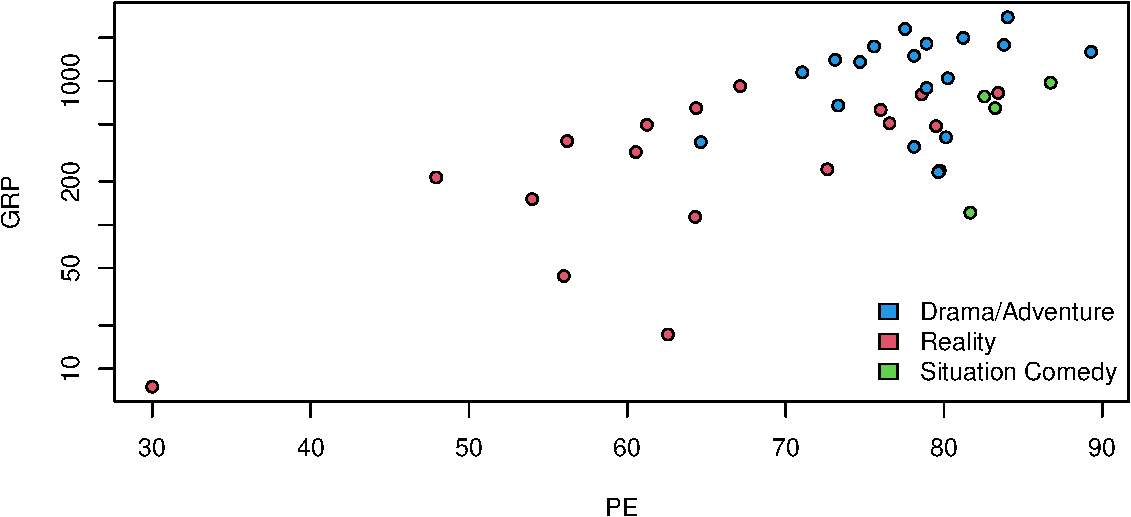
\includegraphics[scale=.7]{figures/unnamed-chunk-1-1.pdf}
 \end{figure}


\end{frame}
%----------------------------------------------------------------------%
\begin{frame}[fragile]
\frametitle{PCR Example: TV Shows}

\begin{itemize}
  \item We have a survey data that include 6241 views and 20 questions for 40 shows. There are two types of questions in the survey. Both ask you the degree to which you agree with a statement. 

\begin{scriptsize}
\begin{Shaded}
\begin{Highlighting}[]
\NormalTok{survey }\OtherTok{\textless{}{-}} \FunctionTok{read.csv}\NormalTok{(}\StringTok{"nbc\_pilotsurvey.csv"}\NormalTok{, }\AttributeTok{as.is=}\ConstantTok{TRUE}\NormalTok{) }
\end{Highlighting}
\end{Shaded}
\end{scriptsize}
\begin{tiny}

\begin{verbatim}
## Rows: 6,241
## Columns: 22
## $ Viewer          <int> 71, 71, 71, 71, 71, 73, 73, 73, 73, 73, 74, 74, 74, 76~
## $ Show            <fct> Iron Chef America, Trading Spaces: All Stars, House Hu~
## $ Q1_Attentive    <int> 3, 4, 4, 4, 4, 2, 4, 3, 2, 5, 4, 4, 4, 3, 3, 4, 5, 4, ~
## $ Q1_Excited      <int> 4, 4, 4, 3, 4, 4, 5, 3, 3, 5, 4, 2, 3, 3, 3, 4, 5, 4, ~
## $ Q1_Happy        <int> 4, 3, 4, 3, 3, 2, 4, 3, 4, 5, 5, 4, 3, 3, 3, 3, 5, 5, ~
## $ Q1_Engaged      <int> 3, 4, 5, 3, 4, 4, 5, 3, 4, 5, 5, 4, 4, 3, 3, 3, 5, 4, ~
## $ Q1_Curious      <int> 5, 5, 5, 4, 4, 2, 5, 4, 4, 5, 4, 4, 5, 4, 2, 3, 5, 3, ~
## $ Q1_Motivated    <int> 4, 2, 3, 2, 4, 3, 3, 4, 2, 5, 4, 3, 4, 3, 1, 3, 2, 2, ~
## $ Q1_Comforted    <int> 3, 3, 3, 2, 3, 3, 2, 2, 3, 4, 5, 2, 3, 2, 1, 1, 2, 3, ~
## $ Q1_Annoyed      <int> 2, 3, 2, 4, 3, 3, 4, 4, 2, 3, 3, 2, 2, 1, 1, 1, 1, 2, ~
## $ Q1_Indifferent  <int> 2, 2, 1, 2, 4, 3, 2, 2, 3, 1, 1, 2, 2, 3, 4, 2, 1, 2, ~
## $ Q2_Relatable    <int> 3, 4, 2, 2, 3, 2, 1, 3, 4, 3, 5, 3, 4, 3, 1, 2, 2, 5, ~
## ...
\end{verbatim}
\end{tiny}

\item The hope is that we can build a rule for predicting viewer interest from pilot surveys, thus helping the studios to make better programming decisions. 
\end{itemize}

\end{frame}
%----------------------------------------------------------------------%
\begin{frame}[fragile]
\frametitle{PCR Example: TV Shows}

\begin{itemize}
  \item It might seem like there is a lot of data here—6241 pilot viewings—but there are only 40 shows and 20 survey questions. 
  \medskip
  \item To relate survey results to show performance, we need to first calculate the average survey question response by show. 
  \medskip
  \item This leads to a 40 × 20 design matrix X, and we can fit PCA on this design.

\end{itemize}
\end{frame}
%----------------------------------------------------------------------%
\begin{frame}[fragile]
\frametitle{PCR Example: TV Shows}


 \begin{figure}[H] \centering
            \captionsetup{justification=centering}
              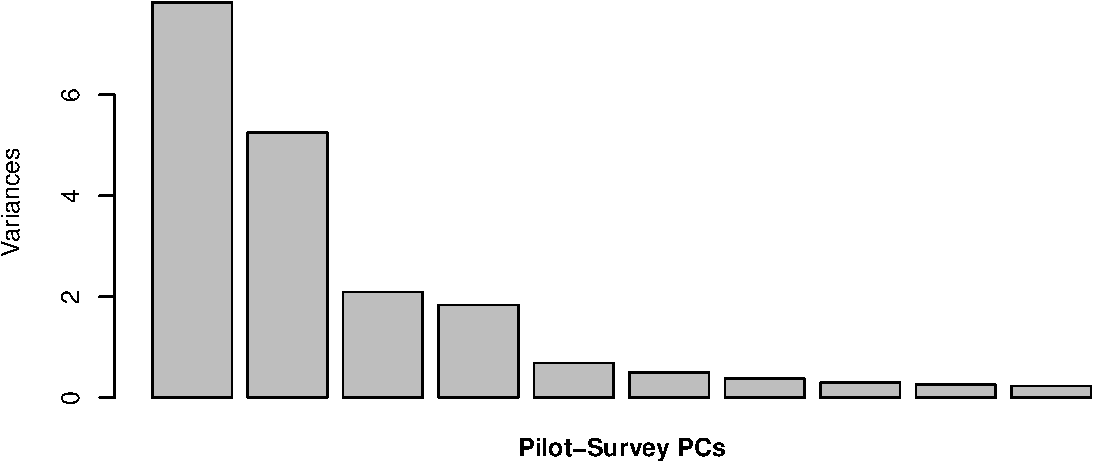
\includegraphics[scale=.5]{figures/unnamed-chunk-3-1.pdf}
 \end{figure}



\end{frame}
%----------------------------------------------------------------------%
\begin{frame}[fragile]
\frametitle{PCR: Example }

\begin{scriptsize}


\begin{Shaded}
\begin{Highlighting}[]
\FunctionTok{round}\NormalTok{(PCApilot}\SpecialCharTok{$}\NormalTok{rotation[,}\DecValTok{1}\SpecialCharTok{:}\DecValTok{3}\NormalTok{],}\DecValTok{1}\NormalTok{)}
\end{Highlighting}
\end{Shaded}
\end{scriptsize}
\begin{tiny}


\begin{verbatim}
##                  PC1  PC2  PC3
## Q1_Attentive    -0.3  0.0  0.0
## Q1_Excited      -0.3  0.1 -0.1
## Q1_Happy        -0.1  0.2 -0.5
## Q1_Engaged      -0.3  0.0  0.0
## Q1_Curious      -0.3  0.0  0.1
## Q1_Motivated    -0.2  0.3  0.0
## Q1_Comforted    -0.1  0.4 -0.1
## Q1_Annoyed       0.2  0.3  0.1
## Q1_Indifferent   0.2  0.4  0.1
## Q2_Relatable    -0.1  0.3 -0.1
## Q2_Funny         0.1  0.2 -0.5
## Q2_Confusing    -0.1  0.3  0.2
## Q2_Predictable   0.2  0.3  0.0
## Q2_Entertaining -0.3 -0.1 -0.3
## Q2_Fantasy      -0.1  0.2  0.1
## Q2_Original     -0.3  0.1 -0.2
## Q2_Believable   -0.1  0.1  0.1
## Q2_Boring        0.2  0.4  0.1
## Q2_Dramatic     -0.2  0.0  0.4
## Q2_Suspenseful  -0.3  0.0  0.3
\end{verbatim}
\end{tiny}
\end{frame}
%----------------------------------------------------------------------%
\begin{frame}[fragile]
\frametitle{PCR: Example }

\begin{scriptsize}

  \begin{Shaded}
  \begin{Highlighting}[]
  \NormalTok{zpilot }\OtherTok{\textless{}{-}} \FunctionTok{predict}\NormalTok{(PCApilot)}

  \end{Highlighting}
  \end{Shaded}
\end{scriptsize}

  \begin{figure}[H] \centering
            \captionsetup{justification=centering}
              
\includegraphics[scale=.5]{figures/unnamed-chunk-5-1.pdf}
 \end{figure}




\end{frame}
%----------------------------------------------------------------------%
\begin{frame}[fragile]
\frametitle{PCR: Example }
\begin{scriptsize}


\begin{Shaded}
\begin{Highlighting}[]
\FunctionTok{library}\NormalTok{(gamlr)}
\NormalTok{PE }\OtherTok{\textless{}{-}}\NormalTok{ shows}\SpecialCharTok{$}\NormalTok{PE}
\NormalTok{zdf }\OtherTok{\textless{}{-}} \FunctionTok{as.data.frame}\NormalTok{(zpilot)}
\FunctionTok{summary}\NormalTok{(PEglm }\OtherTok{\textless{}{-}} \FunctionTok{glm}\NormalTok{(PE }\SpecialCharTok{\textasciitilde{}}\NormalTok{ ., }\AttributeTok{data=}\NormalTok{zdf[,}\DecValTok{1}\SpecialCharTok{:}\DecValTok{2}\NormalTok{]))}
\end{Highlighting}
\end{Shaded}
\end{scriptsize}
\begin{tiny}

\begin{verbatim}
## 
## Call:
## glm(formula = PE ~ ., data = zdf[, 1:2])
## 
## Deviance Residuals: 
##      Min        1Q    Median        3Q       Max  
## -17.7970   -6.6583   -0.7242    6.7524   17.9895  
## 
## Coefficients:
##             Estimate Std. Error t value Pr(>|t|)    
## (Intercept)  72.6831     1.4370  50.580  < 2e-16 ***
## PC1          -2.6401     0.5202  -5.075 1.12e-05 ***
## PC2          -1.5029     0.6349  -2.367   0.0233 *  
## ---
## Signif. codes:  0 '***' 0.001 '**' 0.01 '*' 0.05 '.' 0.1 ' ' 1
## 
## (Dispersion parameter for gaussian family taken to be 82.59648)
## 
##     Null deviance: 5646.5  on 39  degrees of freedom
## Residual deviance: 3056.1  on 37  degrees of freedom
## AIC: 294.96
## 
## Number of Fisher Scoring iterations: 2
\end{verbatim}
\end{tiny}
\end{frame}

%----------------------------------------------------------------------%
\begin{frame}[fragile]
\frametitle{PCR: Example }

\begin{scriptsize}
\begin{Shaded}
\begin{Highlighting}[]
\NormalTok{cvlassoPCR }\OtherTok{\textless{}{-}} \FunctionTok{cv.gamlr}\NormalTok{(}\AttributeTok{x=}\NormalTok{zpilot, }\AttributeTok{y=}\NormalTok{PE, }\AttributeTok{nfold=}\DecValTok{20}\NormalTok{) }\CommentTok{\# nfold=20 for leave{-}two{-}out CV... }
\FunctionTok{coef}\NormalTok{(cvlassoPCR) }
\end{Highlighting}
\end{Shaded}
\end{scriptsize}

\begin{tiny}
\begin{verbatim}
## 21 x 1 sparse Matrix of class "dgCMatrix"
##                seg28
## intercept 72.6830750
## PC1       -1.8881753
## PC2       -0.5852612
## PC3       -0.7950954
## PC4        .        
## PC5        .        
## PC6        .        
## PC7       -3.1873761
## PC8        .        
## PC9        .        
## PC10       .        
## PC11       .        
## PC12       .        
## PC13       .        
## PC14       .        
## PC15       .        
## PC16      10.0701768
## PC17       .        
## PC18       .        
## PC19       .        
## PC20       .
\end{verbatim}
\end{tiny}
\end{frame}

%----------------------------------------------------------------------%
\begin{frame}[fragile]
\frametitle{PCR: Example }


 \begin{figure}[H] \centering
            \captionsetup{justification=centering}
              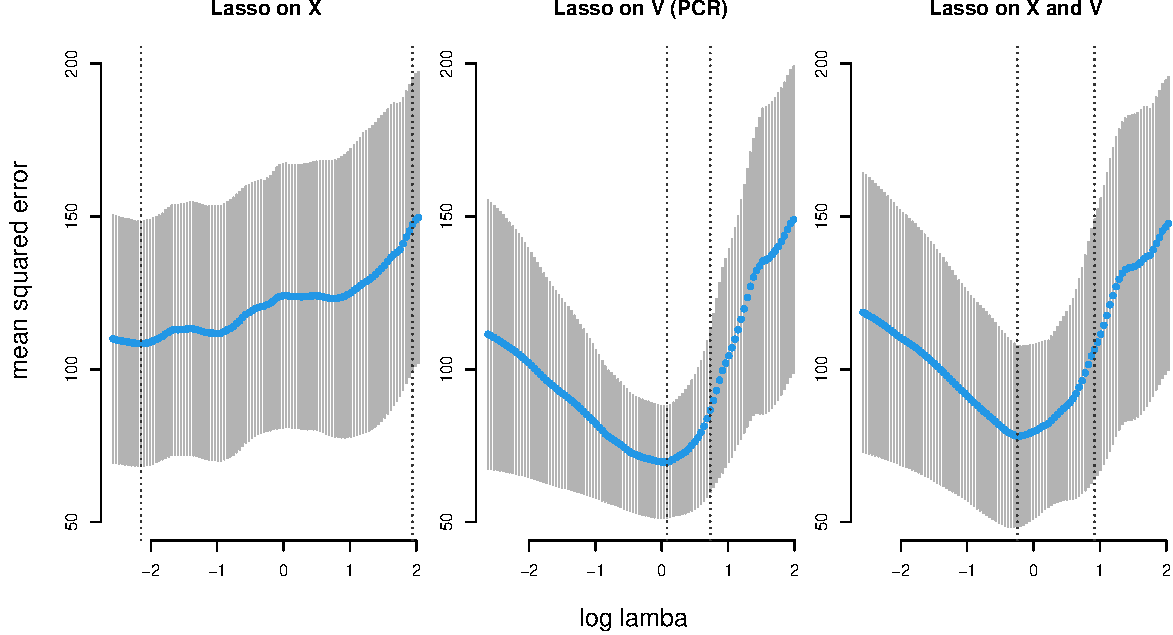
\includegraphics[scale=.6]{figures/unnamed-chunk-9-1.pdf}
 \end{figure}



\end{frame}
%----------------------------------------------------------------------%
\section{Partial Least Squares }
%----------------------------------------------------------------------%
\begin{frame}[fragile]
\frametitle{Partial Least Squares }

\begin{itemize}
\item In the previous two examples, there was a clear low-dimensional factor structure in $X$: ideology in Congress and like-versus-dislike in the TV pilot survey. 
\medskip
\item  For the TV pilots, these factors were also directly related to the $y$ response of interest. 
\medskip
\item  Nature will not always be this nice. It is common to encounter $X$ data that has been generated without a clear factor structure, or through some messy mix of underlying factors and idiosyncratic shocks. 
\medskip
\item And even when there is factor structure in $X$, it will often be that $y$ is not related to the dominant sources of variation in $X$. 
\medskip
\item The response is not driven by the first few PCs, and it is inefficient to try to estimate $f$ as a middle-man between $y$ and $X$. 

\end{itemize}

\end{frame}
%----------------------------------------------------------------------%
\section{Partial Least Squares }
%----------------------------------------------------------------------%
\begin{frame}[fragile]
\frametitle{Partial Least Squares }

\begin{itemize}

\item  PCR will work only if the dominant directions of variation in $X$ are related to $y$.
\medskip
\item  However, the idea of combining inputs into a few factors (or indices) that affect $y$ is an appealing framework. 
\medskip
\item Is there a way to force factors $f$ to be relevant to both $X$ and $y$? 
\end{itemize}

\end{frame}
%----------------------------------------------------------------------%
\begin{frame}[fragile]
\frametitle{Partial Least Squares }

\begin{itemize}
\item Yes; 
\medskip
\pause
\item It's known as supervised factor modeling, and it is a useful big data technique. 
\medskip
\item There is a big world of supervised factor modeling, and there are several algorithms for supervised adaptations of PCA.
\medskip
\item  We’ll consider the simple but powerful method of partial least squares (PLS)

\medskip
\item  To understand PLS, we start with the more basic algorithm of marginal regression (MR).
\end{itemize}

\end{frame}
%----------------------------------------------------------------------%
\subsection{Marginal Regression (MR)}
%----------------------------------------------------------------------%
\begin{frame}[fragile]
\frametitle{Marginal Regression (MR)}

\begin{itemize}
  \item  Idea,
  \begin{enumerate}
    \item Run $y\Rightarrow$ on each $X$
    \item Use the coefficients to map from $X$ to a univariate factor F
  \end{enumerate}
  \medskip
   \item This factor aggregates the first-order effect of each input variable on y. 
  \medskip
\item It will be dominated by $X_j$ dimensions that both 
\begin{enumerate}
\item  have a big effect on $y$ 
\item  move consistently in the same direction with each other (since their influence on the factor is additive). 
\end{enumerate}
\medskip
\item That is, marginal regression constructs a single factor that is connected both to $y$ and to a dominant direction of variation in $X$. 
\end{itemize}

\end{frame}

%----------------------------------------------------------------------%
\begin{frame}[fragile]
\frametitle{Marginal Regression (MR)}

\begin{itemize}
\item MR Algorithm
\medskip
\begin{enumerate}
  \item Calculate $\delta=(\delta_1,...,\delta_n)$ where $\delta_j = cor (X_j, y)/sd(X_j)$ is the OLS coefficient in a simple univariate regression for $y$ on $X_j$. 
  \medskip
  \item Set $f_i = X'_i\delta = \sum_j X_{ij} \delta_j$ for each observation i. 
  \medskip
  \item Fit the “forward” univariate linear regression $y_i = \alpha + \beta f_i + \epsilon_i$
  \medskip
  \item Given a new $X$,we can predict $\hat{y}=\hat{\alpha} + \hat{\beta} X'\delta$
\end{enumerate}

\end{itemize}

\end{frame}

%----------------------------------------------------------------------%
\begin{frame}[fragile]
\frametitle{Marginal Regression (MR)}

\begin{itemize}

\item One big advantage of MR is computational efficiency. 
\medskip
\item We can use MapReduce:
\medskip
\begin{itemize}
\item In the Map step, you produce $(x_{ij}, y_i)$ pairs that are indexed by the dimension key j; 
\medskip
\item the Reduce step then runs univariate OLS for y on $x_j$ and returns $\delta_j$. 
\medskip
\end{itemize}
\item It works in high dimensions even if $p >> n$.
\medskip
\item MR is a strategy for supervised learning in ultra-high dimensions.
\end{itemize} 


\end{frame}
%----------------------------------------------------------------------%
\begin{frame}[fragile]
\frametitle{Partial Least Squares }

\begin{itemize}
\item Partial least squares (PLS) is an extension of marginal regression.
\pause 
\medskip
\item  Instead of stopping after running the single MR, you iterate: 
\medskip
\begin{itemize}
  \item Take the residuals from the first MR and repeat a second MR to predict these residuals. 
  \medskip
  \item You can then take the residuals from the second MR and repeat, continuing until you reach the minimum of p and n. 
\end{itemize}
\end{itemize}
\end{frame}
%----------------------------------------------------------------------%
\begin{frame}[fragile]
\frametitle{Partial Least Squares }

\begin{itemize}
\item PLS Algorithm 
\medskip
\begin{enumerate}
\item Begin by running MR algorithm as before for y on X.
\medskip 
\item Store the MR factor as $f_1$, the 1st PLS direction, and PLS(1) forward regression fitted values as $\hat{y}_1=\alpha + \beta_1 f_1)$
\medskip 
\item Then, for k = 2, ... K, calculate the following:    
  \begin{itemize}
    \item Residuals     
    \item Loadings     
    \item Fitted values 
  \end{itemize}
\item This yields PLS rotations $\delta=(\delta_1,...,\delta_k)$ and factors $F=(f_1,...,f_k)$.
\end{enumerate}
\end{itemize}

\end{frame}
%----------------------------------------------------------------------%
\begin{frame}[fragile]
\frametitle{Partial Least Squares }

\begin{itemize}
  \item This yields PLS rotations $\delta=(\delta_1,...,\delta_k)$ and factors $F=(f_1,...,f_k$.
\medskip 
\item The PLS algorithm involves a number of steps but is really very simple.
\medskip 
\item  We are just running marginal regression on the residuals after each PLS(k) fit and updating the fitted values.
\medskip 
 \item   This general procedure of taking a simple algorithm and repeatedly applying it to residuals from previous fits. (This is boosting!!) 
\end{itemize}


\end{frame}
%----------------------------------------------------------------------%
\begin{frame}[fragile]
\frametitle{Partial Least Squares }

\begin{itemize}
\item If $p < n$ and you do PLS with $K = p$, then the fitted $\hat{y}^K_i$ will be the same as what you would get running OLS for $y$ on $X$.
\medskip
\item The PLS coefficients on each $X_{i}$, available as $\sum_k \beta_{k} \delta_{kj}$, also match the OLS coefficients. 
\medskip
\item Thus, PLS provides a path of models between MR and OLS.
\medskip
 \item Remember whenever you are boosting, there is a potential for overfit. 
\end{itemize}

\end{frame}

%----------------------------------------------------------------------%
\begin{frame}[fragile]
\frametitle{Text Regression: Example (Gentzkow and Shapiro)}
\begin{scriptsize}



\begin{Shaded}
\begin{Highlighting}[]
\CommentTok{\#load packages}
\KeywordTok{library}\NormalTok{(textir) }
\CommentTok{\#load data}
\KeywordTok{data}\NormalTok{(congress109)}
\NormalTok{congress109Counts[}\KeywordTok{c}\NormalTok{(}\StringTok{"Barack Obama"}\NormalTok{,}\StringTok{"John Boehner"}\NormalTok{),}\DecValTok{995}\OperatorTok{:}\DecValTok{998}\NormalTok{]}
\end{Highlighting}
\end{Shaded}

\end{scriptsize}
\begin{tiny}


\begin{verbatim}
## 2 x 4 sparse Matrix of class "dgCMatrix"
##              stem.cel natural.ga hurricane.katrina trade.agreement
## Barack Obama        .          1                20               7
## John Boehner        .          .                14               .
\end{verbatim}

\end{tiny}
\begin{scriptsize}


\begin{Shaded}
\begin{Highlighting}[]
\NormalTok{congress109Ideology[}\DecValTok{1}\OperatorTok{:}\DecValTok{4}\NormalTok{,}\DecValTok{1}\OperatorTok{:}\DecValTok{5}\NormalTok{]}
\end{Highlighting}
\end{Shaded}
\end{scriptsize}
\begin{tiny}


\begin{verbatim}
##                            name party state chamber  repshare
## Chris Cannon       Chris Cannon     R    UT       H 0.7900621
## Michael Conaway Michael Conaway     R    TX       H 0.7836028
## Spencer Bachus   Spencer Bachus     R    AL       H 0.7812933
## Mac Thornberry   Mac Thornberry     R    TX       H 0.7776520
\end{verbatim}
\end{tiny}
\end{frame}

%----------------------------------------------------------------------%
\begin{frame}[fragile]
\frametitle{Text Regression: Example (Gentzkow and Shapiro)}

\begin{itemize}
  \item We used {\tt LASSO} and got
\end{itemize}
\begin{scriptsize}

\begin{Shaded}
\begin{Highlighting}[]
\KeywordTok{head}\NormalTok{(}\KeywordTok{sort}\NormalTok{(}\KeywordTok{round}\NormalTok{(B[B}\OperatorTok{!=}\DecValTok{0}\NormalTok{],}\DecValTok{4}\NormalTok{)),}\DecValTok{10}\NormalTok{)}
\end{Highlighting}
\end{Shaded}

\end{scriptsize}
\begin{tiny}


\begin{verbatim}
##    congressional.black.caucu                 family.value 
##                      -0.0839                      -0.0443 
##        issue.facing.american           voter.registration 
##                      -0.0324                      -0.0298 
##      minority.owned.business            strong.opposition 
##                      -0.0284                      -0.0264 
##                  civil.right        universal.health.care 
##                      -0.0259                      -0.0254 
## congressional.hispanic.caucu          ohio.electoral.vote 
##                      -0.0187                      -0.0183
\end{verbatim}
\end{tiny}

\begin{scriptsize}

\begin{Shaded}
\begin{Highlighting}[]
\KeywordTok{tail}\NormalTok{(}\KeywordTok{sort}\NormalTok{(}\KeywordTok{round}\NormalTok{(B[B}\OperatorTok{!=}\DecValTok{0}\NormalTok{],}\DecValTok{4}\NormalTok{)),}\DecValTok{10}\NormalTok{)}
\end{Highlighting}
\end{Shaded}

\end{scriptsize}
\begin{tiny}

\begin{verbatim}
##         illegal.alien        percent.growth   illegal.immigration 
##                0.0079                0.0083                0.0087 
##            global.war          look.forward            war.terror 
##                0.0098                0.0099                0.0114 
##      private.property        action.lawsuit          human.embryo 
##                0.0133                0.0142                0.0226 
## million.illegal.alien 
##                0.0328
\end{verbatim}


\end{tiny}

\end{frame}

%----------------------------------------------------------------------%
\begin{frame}[fragile]
\frametitle{Text Regression: Example (Gentzkow and Shapiro)}

\begin{scriptsize}
\begin{Shaded}
\begin{Highlighting}[]

\NormalTok{slant }\OtherTok{\textless{}{-}} \FunctionTok{pls}\NormalTok{(f, y, }\AttributeTok{K=}\DecValTok{3}\NormalTok{)}
\end{Highlighting}
\end{Shaded}
\end{scriptsize}
\begin{tiny}
\begin{verbatim}
## Directions 1, 2, 3, done.
\end{verbatim}
\end{tiny}


  \begin{figure}[H] \centering
            \captionsetup{justification=centering}
              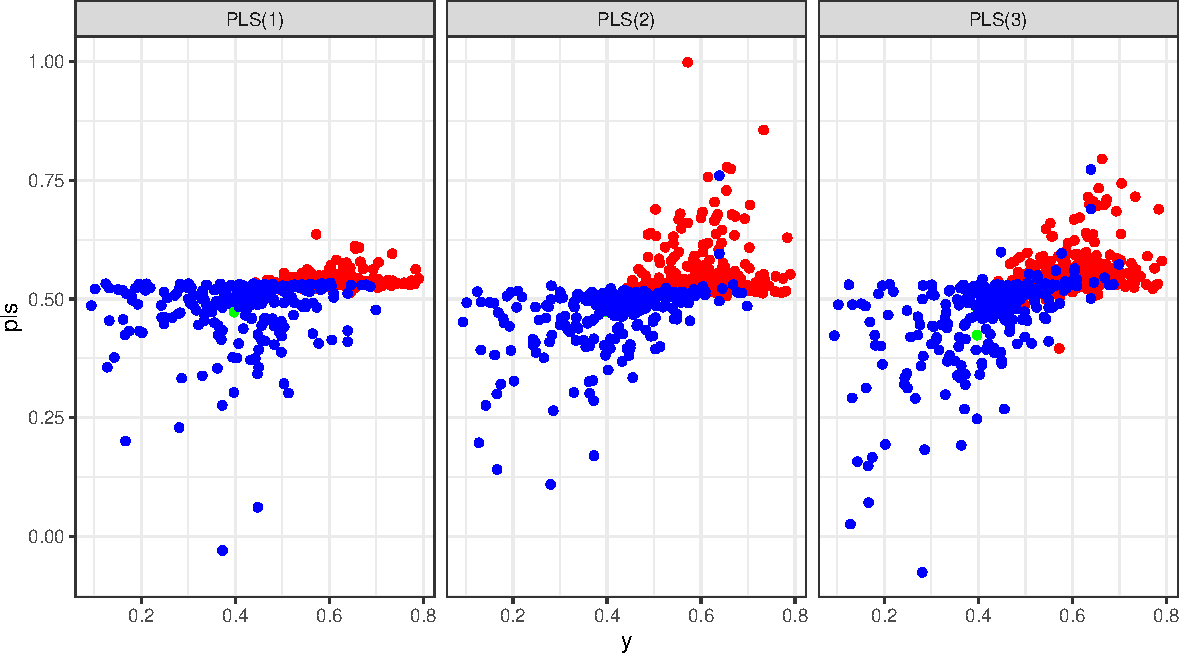
\includegraphics[scale=.5]{figures/pls.pdf}
 \end{figure}


\end{frame}

%----------------------------------------------------------------------%
\begin{frame}[fragile]
\frametitle{Text Regression: Example (Gentzkow and Shapiro)}

\begin{figure}%
    \centering
    \subfloat[\centering MSE PLS]{{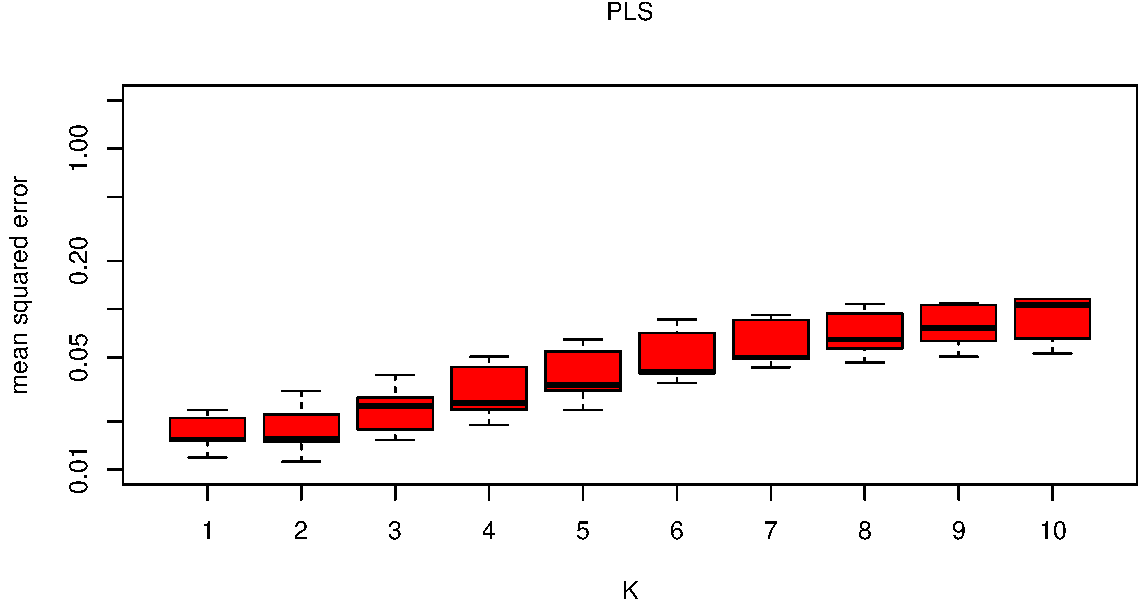
\includegraphics[width=7cm, height=6cm]{figures/mse_pls.pdf} }}%
    \qquad
    \subfloat[\centering MSE  Lasso]{{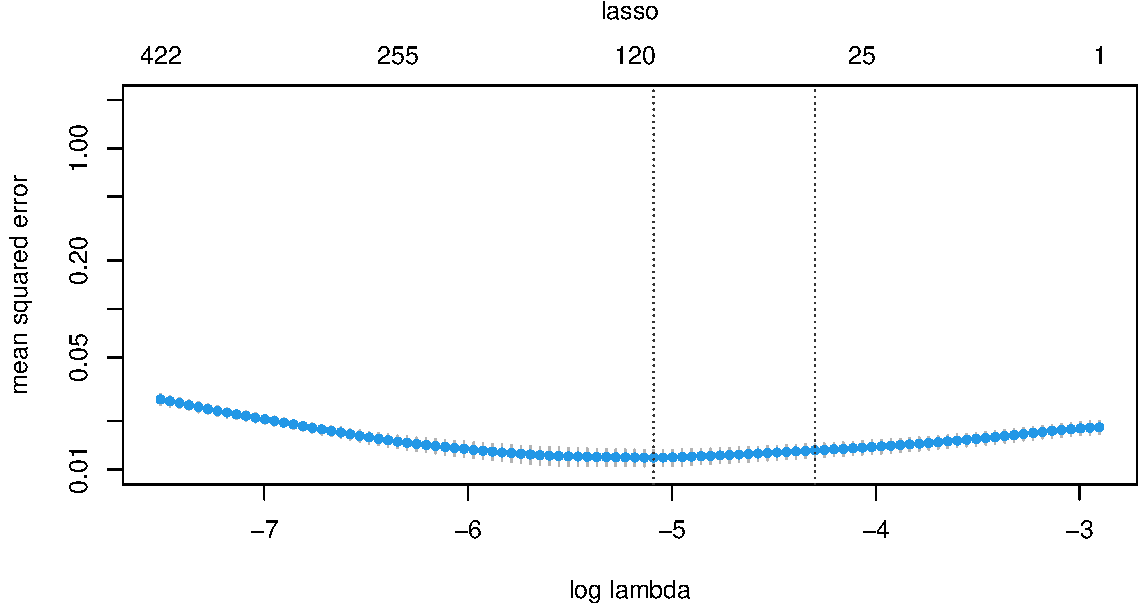
\includegraphics[width=7cm, height=6cm]{figures/mse_lasso.pdf} }}%
    %\caption{2 Figures side by side}%
    %\label{fig:example}%
\end{figure}

\end{frame}

%----------------------------------------------------------------------%
\section{Review
 \& Next Steps}
%----------------------------------------------------------------------%
\begin{frame}
\frametitle{Review \& Next Steps}
  
\begin{itemize} 
  

\medskip
\item Factor Models: Example PCA
    \bigskip  
  \item  Next class:  
  \begin{itemize}
  \item Presentation Rafael
    \medskip
    \item Word Embedings
  \end{itemize}


\bigskip  
\item Questions? Questions about software? 

\end{itemize}
\end{frame}

%----------------------------------------------------------------------%
\section{Further Readings}
%----------------------------------------------------------------------%
\begin{frame}
\frametitle{Further Readings}

\begin{itemize}

  \item Gentzkow, M., \& Shapiro, J. M. (2010). What drives media slant? Evidence from US daily newspapers. Econometrica, 78(1), 35-71.
  \medskip
  \item Friedman, J., Hastie, T., \& Tibshirani, R. (2001). The elements of statistical learning (Vol. 1, No. 10). New York: Springer series in statistics.
  \medskip
  \item James, G., Witten, D., Hastie, T., \& Tibshirani, R. (2013). An introduction to statistical learning (Vol. 112, p. 18). New York: springer.
  \medskip
  \item Taddy, M. (2019). Business data science: Combining machine learning and economics to optimize, automate, and accelerate business decisions. McGraw Hill Professional.

  
\end{itemize}

\end{frame}
%----------------------------------------------------------------------%
%----------------------------------------------------------------------%
\end{document}
%----------------------------------------------------------------------%
%----------------------------------------------------------------------%

